\section{LLM whiteboard}



\begin{figure}[h]
    \centering
    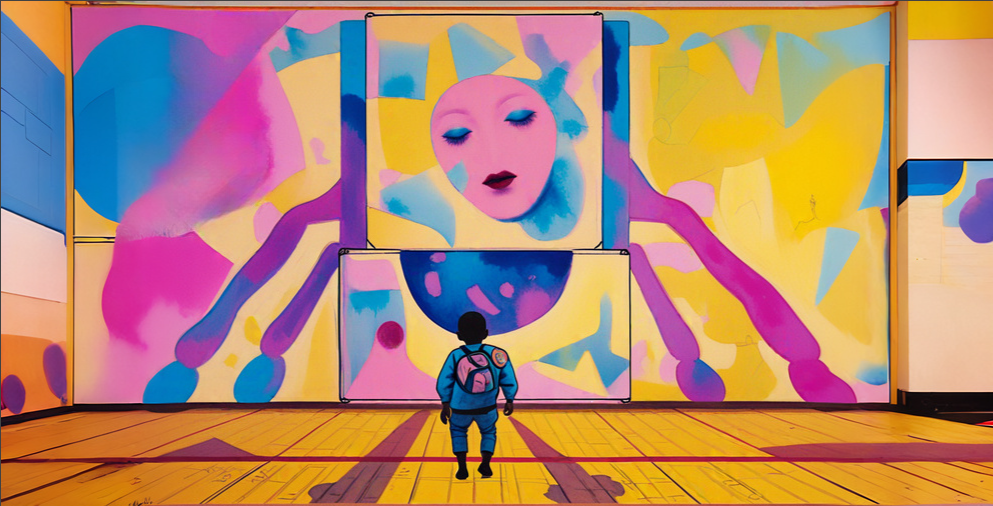
\includegraphics[width=\textwidth]{wBaordBanner.png}
    \caption{The spirit of the LLM WhiteBoard platform.}
    \vspace{0.1cm}
    \label{fig:spiritofWB}
\end{figure}

% \subsection{Collaborative Paradigms in AI and HCI}

\subsubsection{Exploring Spatial and Semantic Interfaces}
The intersection of Human-Computer Interaction (HCI) and artificial intelligence has seen significant transformations with the advent of large language models (LLMs) acting as semantic operators.
These models bridge the gap between human intent and machine action, allowing users to interact with systems through high-level commands.
This paradigm enables more abstract, fluid interaction—users no longer need to micromanage interfaces but can instead provide overarching directives that the AI interprets and translates into executable code.
However, an equally important element in modern HCI design is the spatial aspect of collaboration, as seen in Spatial Pixel's work.
This combination of semantic understanding and spatial interaction is reshaping how we think about digital experiences.

\subsubsection{SpatialPixel and the Evolution of Digital Collaboration}
Traditional digital interfaces, largely confined to flat screens, often limit the user’s ability to engage with systems in meaningful ways.
This issue, sometimes referred to as "flat screen, flat thoughts,"\cite{whitney2024} highlights how modern interfaces—designed around two-dimensional layouts—can stifle creativity and limit interaction.
Violet Whitney and William Martin, through their work at Spatial Pixel, advocate for a more spatial approach to interface design.
They argue that human cognition is inherently spatial and embodied; our thoughts, behaviors, and problem-solving processes are deeply influenced by how we organize our physical environments.
In contrast to traditional screen-based systems, spatial interfaces allow users to leverage their embodied cognition, enhancing the possibilities for creative expression and complex problem solving.

SpatialPixel's work illustrates how knowledge work, much like manual labor, is inherently spatial.
Tools like Miro and Mural brought attention to this by allowing users to zoom out and organize tasks spatially on a canvas, mimicking how we naturally organize our workspaces in the physical world.
This concept of spatial cognition—the idea that we think through the space around us—provides an essential framework for the development of more immersive, AI-enhanced digital experiences.

\begin{figure}[h]
    \centering
    
\includegraphics[width=\textwidth/3]{spatialpixel.png}
    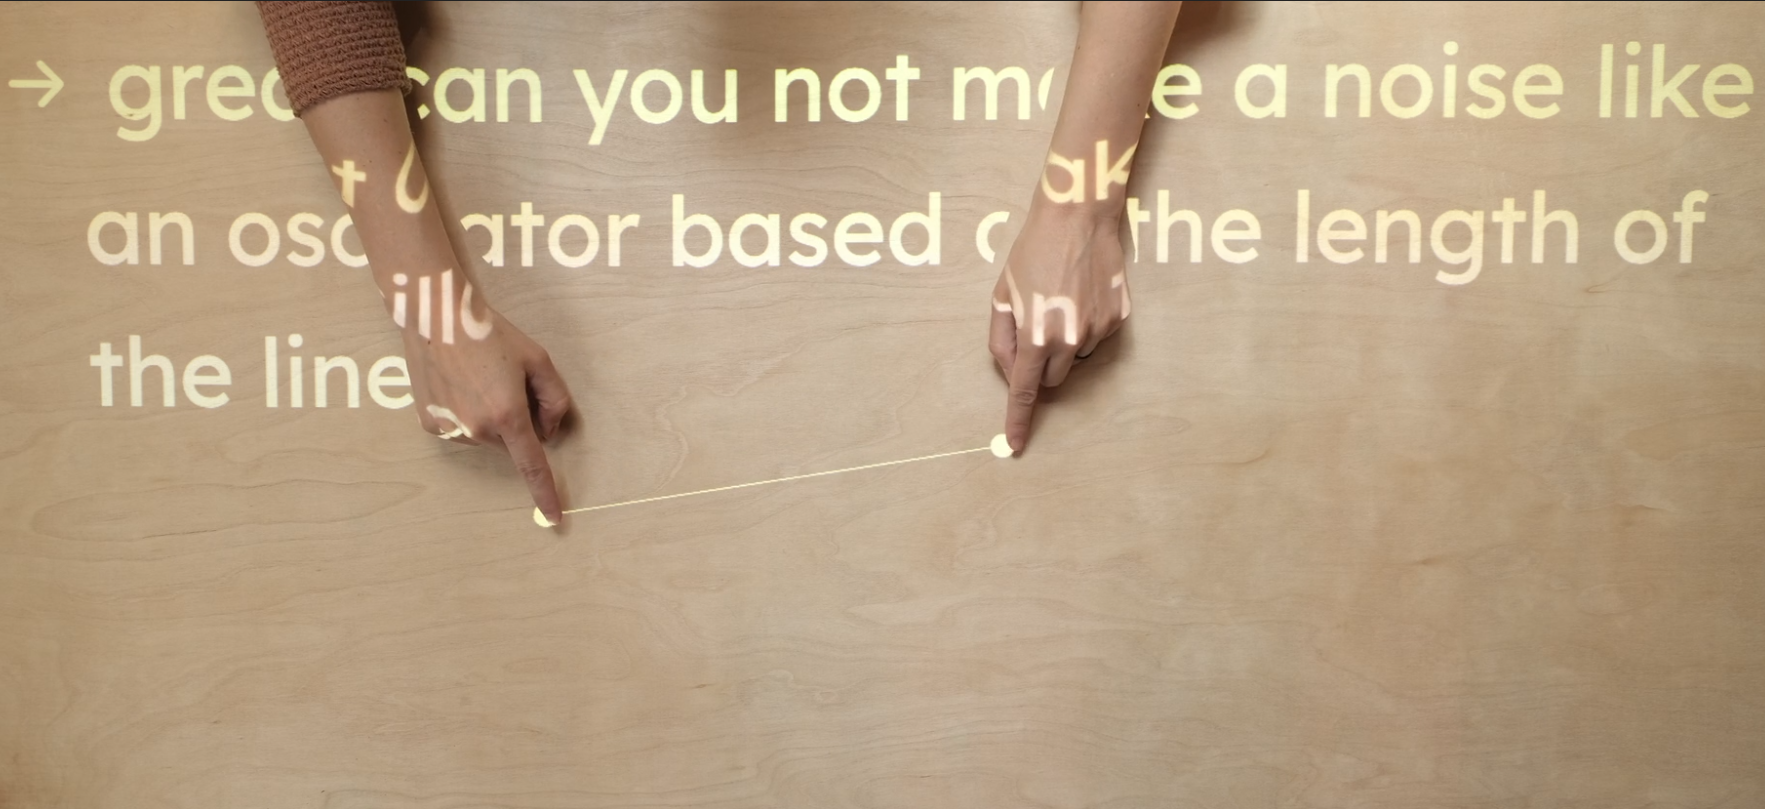
\includegraphics[width=\textwidth/3]{spatialpixel2.png}
    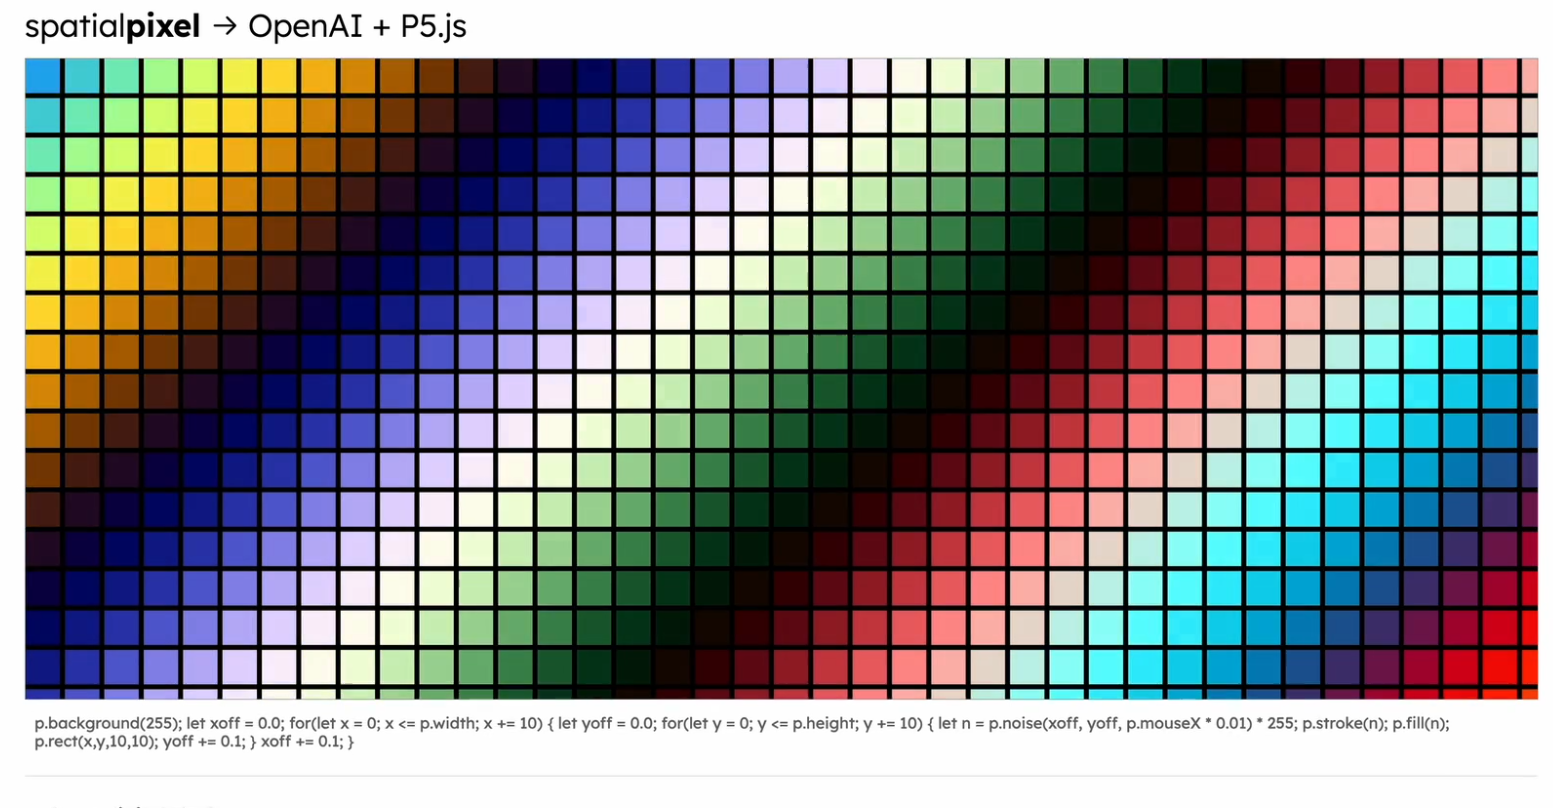
\includegraphics[width=\textwidth/3]{spatialpiwel3.png}
    \caption{Showcase of SpatialPixel's work on integrating spatial paradigms in LLM assisted applications.}
    \vspace{0.1cm}
    \label{fig:spatialpixel}
\end{figure}

The LLM Whiteboard project builds on these principles by combining the semantic power of LLMs with spatial interaction.
Users can issue commands to the LLM, which generates dynamic graphical elements within a p5.js environment.
This interaction becomes even more powerful when combined with spatial technologies, as demonstrated by the AR mode, where users can manipulate digital entities in real-world environments using Mediapipe.
Here, the spatial relationships between entities are not only visual but embodied, allowing users to interact with the system in ways that align with their natural cognitive processes.

For example, in the AR mode of the LLM Whiteboard, a user can point to a location within their physical environment, and the LLM, using Mediapipe, generates a corresponding digital entity in real-time. This interaction mimics how we naturally manipulate physical objects, further aligning the interface with the user’s cognitive expectations. By introducing spatiality into the interaction, the system enables a more intuitive and expansive form of collaboration, where both the LLM and the user co-create in a shared physical-digital space.


\subsubsection{Integrating LLMs with Spatial Intelligence}
By incorporating both semantic and spatial affordances, the LLM Whiteboard project creates a novel paradigm for collaborative digital interaction.
LLMs, as semantic operators, can handle high-level directives, translating abstract user inputs into specific actions.
At the same time, spatial technologies like Mediapipe allow for embodied interactions, grounding those digital actions in physical space.
This dual approach enables what can be described as low-signaling, high-possibility affordances—the system requires minimal input from the user to generate complex and meaningful outputs, while also allowing for expansive, freeform interactions that align with natural human cognition.

The integration of spatial computing further extends the collaborative possibilities by allowing users to offload cognitive tasks into the environment.
This aligns with the Extended Mind Theory, which suggests that cognitive processes are not confined to the brain but are distributed across the body and environment through the use of external tools.
LLMs, in this sense, serve as epistemic artifacts, tools that extend our ability to process information, while spatial interaction provides the physical grounding needed for effective problem-solving and creativity.


\subsection{The Role of Semantic Operators in AI-Driven Autonomy}
Large language models (LLMs) are increasingly acting as semantic operators—intelligent systems that bridge the gap between human intent and machine execution.
In this role, LLMs interpret high-level commands and autonomously generate corresponding actions, offering new possibilities for user interaction.
This shift from explicit command-based interactions to abstract, semantic-level collaboration represents a significant evolution in HCI, reducing the cognitive load on users while expanding their creative capabilities.

This section introduces key technologies, like Langchain\cite{chase2022}, that support the operation of LLMs as semantic operators, and integrates a discussion of current advancements in AI-driven autonomy, exemplified by AutoGPT\cite{autogpt2024}, BabyAGI\cite{nakajima2024}, and Microsoft Research’s “Sparks of Artificial General Intelligence” paper\cite{bubeck2023sparks}.
These developments collectively shape the way we understand how LLMs operate in complex digital systems, scaling their semantic capabilities and pushing toward broader, autonomous applications.

\subsubsection{LLMs as Semantic Operators}
At the core of the LLM Whiteboard project is the concept of LLMs functioning as semantic operators.
Rather than requiring explicit, low-level programming input, these models enable users to interact at a higher, more abstract level.
By processing human commands in natural language, LLMs act as intermediaries, translating user intent into executable actions or code.
This allows for the exploration of new forms of creative collaboration, where users are empowered to direct processes without the need for technical knowledge.

In this context, the concept of low-signaling, high-possibility affordances becomes central.
With minimal input from users—such as a simple command to "create a moving circle"—the LLM can generate complex, dynamic systems within a live coding environment.
Using technologies like p5.js for graphics and Langchain for tool orchestration, these models can handle complex digital tasks, manage the execution of various functions, and even self-correct through feedback loops.

\subsubsection{Langchain: Operationalizing LLMs as Semantic Operators}
The technological backbone that enables LLMs to function as semantic operators in the LLM Whiteboard project is Langchain.
Langchain serves both as a framework and an operational paradigm, allowing LLMs to orchestrate complex workflows by integrating various external tools and APIs.
In the case of the LLM Whiteboard, Langchain allows the model to dynamically access and manipulate graphical entities in p5.js while also handling error correction and iteration.

Langchain transforms LLMs into tool-driven operators, where the model intelligently selects the most appropriate resources for the task at hand.
For example, when the LLM is asked to "create a bouncing ball," it can automatically generate the necessary code in p5.js while simultaneously managing the visual attributes and behaviors of the entity.
Langchain’s orchestration of tools enables LLMs to perform complex tasks across multiple domains, making them more autonomous and capable of handling diverse user inputs in real-time.

Beyond its immediate application in the LLM Whiteboard, Langchain provides the foundation for scaling LLM-based systems into more sophisticated autonomous agents.
These agents, which we will explore in more detail, extend the operational scope of LLMs, allowing them to handle increasingly complex and large-scale tasks.

\subsubsection{The Sea of LLM Agents: Scaling Semantic Capabilities}
As LLMs become more powerful, they evolve from standalone operators into distributed systems of LLM agents.
Each agent can specialize in different aspects of the task, collaborating with others to achieve higher complexity and scalability.
This concept of a sea of LLM agents, orchestrated through frameworks like Langchain, opens up vast possibilities for building autonomous systems that can perform tasks traditionally associated with human intelligence.

In the LLM Whiteboard project, this could involve multiple agents working in parallel—some handling the generation of graphical entities, others managing the interaction with external APIs, and yet another agent responsible for debugging and iterating on user feedback.
By decentralizing the task management process, the system becomes more flexible, scalable, and capable of handling complex workflows.

The emergence of autonomous multi-agent systems is emblematic of a broader trend in AI, as demonstrated by recent innovations like AutoGPT and BabyAGI.

\subsubsection{State of the Art: AutoGPT, BabyAGI, and Sparks of AGI}
The development of AutoGPT and BabyAGI offers a glimpse into how LLMs are being used as autonomous agents capable of handling complex tasks with minimal user input.
These systems represent the next step in scaling the semantic capabilities of LLMs, turning them into self-governing entities capable of multi-step reasoning, task decomposition, and even learning from experience.

\textbf{AutoGPT} demonstrates how LLMs can autonomously manage and complete tasks by breaking down high-level goals into subtasks and iterating over them without constant human guidance.
In a system like AutoGPT, LLMs go beyond responding to user prompts—they actively take on goals, strategize solutions, and execute actions autonomously.
This aligns with the goals of the LLM Whiteboard project, which seeks to minimize user input while maximizing creative output, allowing users to provide abstract commands that the model turns into executable code.

\textbf{BabyAGI} takes a learning-oriented approach to autonomy, focusing on task-oriented learning and recursive improvement.
This system simulates early stages of Artificial General Intelligence (AGI) by using feedback loops to iteratively improve its performance on tasks.
For the LLM Whiteboard, integrating BabyAGI-like capabilities would mean the system could learn from user interactions, refining its output based on real-time feedback.
This would enhance the model's ability to act as a creative partner, adapting to user preferences and improving its code generation over time.

\textbf{Sparks of AGI}, the paper published by Microsoft Research, explores the theoretical underpinnings of AGI, suggesting that LLMs are beginning to show early signs of general intelligence.
This research underlines the importance of multi-step reasoning and adaptability, features that are increasingly becoming part of systems like AutoGPT and BabyAGI.
The paper's insights reinforce the potential for LLMs to act as powerful semantic operators capable of handling complex, open-ended tasks that go beyond narrow use cases.

\subsubsection{Impact on the LLM Whiteboard Project}
The advances demonstrated by AutoGPT, BabyAGI, and the “Sparks of AGI” paper directly influence the trajectory of the LLM Whiteboard project.
As we integrate these cutting-edge concepts, we move toward a future where LLMs can serve as true creative collaborators, autonomously managing the complex digital experiences envisioned by users.
The incorporation of Langchain and the potential for multi-agent architectures allows the LLM Whiteboard to handle increasingly sophisticated design tasks with minimal intervention, reflecting the principles of low-signaling, high-possibility affordances in HCI.

By leveraging the operational power of autonomous agents, the LLM Whiteboard can expand its capabilities to include task learning, multi-agent collaboration, and iterative improvement.
This positions the project not just as a creative tool, but as a model for future systems that blend user-driven interaction with AI-driven autonomy, unlocking new possibilities for large-scale, adaptive digital experiences.

By incorporating the latest advances in AI-driven autonomy and task execution, the project demonstrates the profound potential of LLMs to act as powerful semantic operators—agents capable of transforming abstract user inputs into dynamic, creative outputs at scale.

\subsection{ Implementation of LLM Whiteboard}

The technical framework of the LLM Whiteboard revolves around two core technologies: Langchain and p5.js.

Langchain is a language model orchestration framework that facilitates the integration of tools, APIs, and databases with LLMs.
Within the LLM Whiteboard, Langchain enables the model to access various tools, allowing for a fluid interaction between user commands and the model's code generation capabilities.
By structuring prompts and defining tools that LLMs can use, Langchain serves as the backbone for zero-shot prompting, ensuring that the model can generate new entities and functions on the fly.
This architecture also supports the fallback mechanism, allowing the model to correct and iterate on its own code in real-time.

p5.js provides the graphical environment where the LLM Whiteboard brings user commands to life.
A JavaScript library designed for creative coding, p5.js offers an intuitive framework for generating interactive graphics.
The LLM uses this library to instantiate and manipulate entities like circles, rectangles, or more complex forms, linking abstract user inputs to visual outputs.
p5.js’s ability to handle real-time animations and dynamic user interactions makes it an ideal platform for this form of AI-assisted creation.
Additionally, the LLM can extend p5.js's core functionality by writing custom functions that augment the library’s capabilities, further expanding the creative space available to the user.

\begin{figure}[h!]
    \centering
    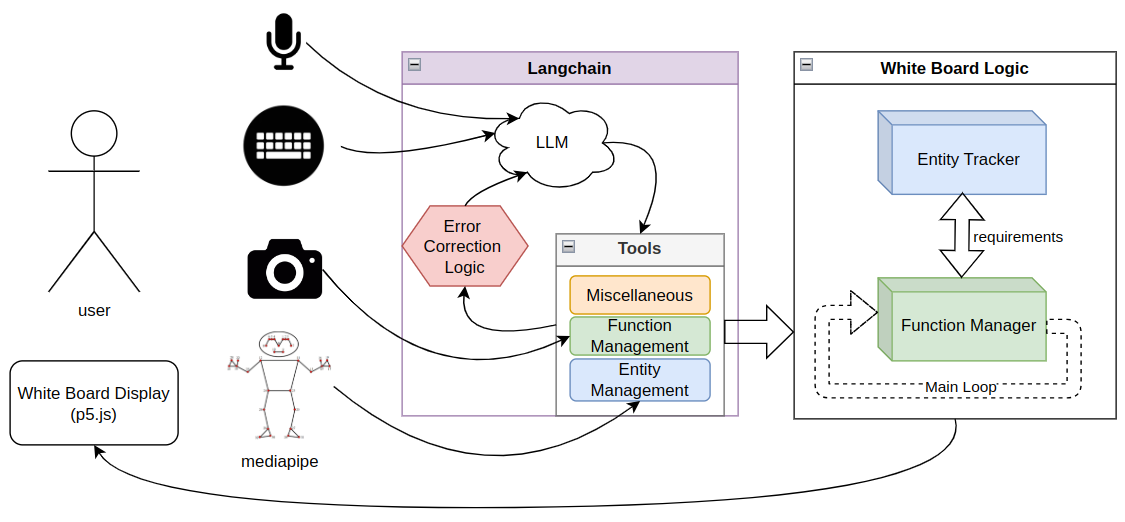
\includegraphics[width=\textwidth]{llmwhiteboard.drawio.png}
    \caption{Architecture diagram of the LLM WhiteBoard.}
    \vspace{0.1cm}
    \label{fig:wbarchietcure}
\end{figure}

Together, these technologies form the foundation of a system that combines user-driven creativity with the autonomous problem-solving abilities of LLMs.
The LLM Whiteboard thus stands as a demonstration of how AI can enable new forms of interaction in HCI, allowing users to explore high-possibility, low-signaling affordances that lower the barrier to creative expression while expanding the range of what can be accomplished with minimal input.

\subsubsection{ How It All Comes Together}


\begin{figure}[h!]
    \centering
    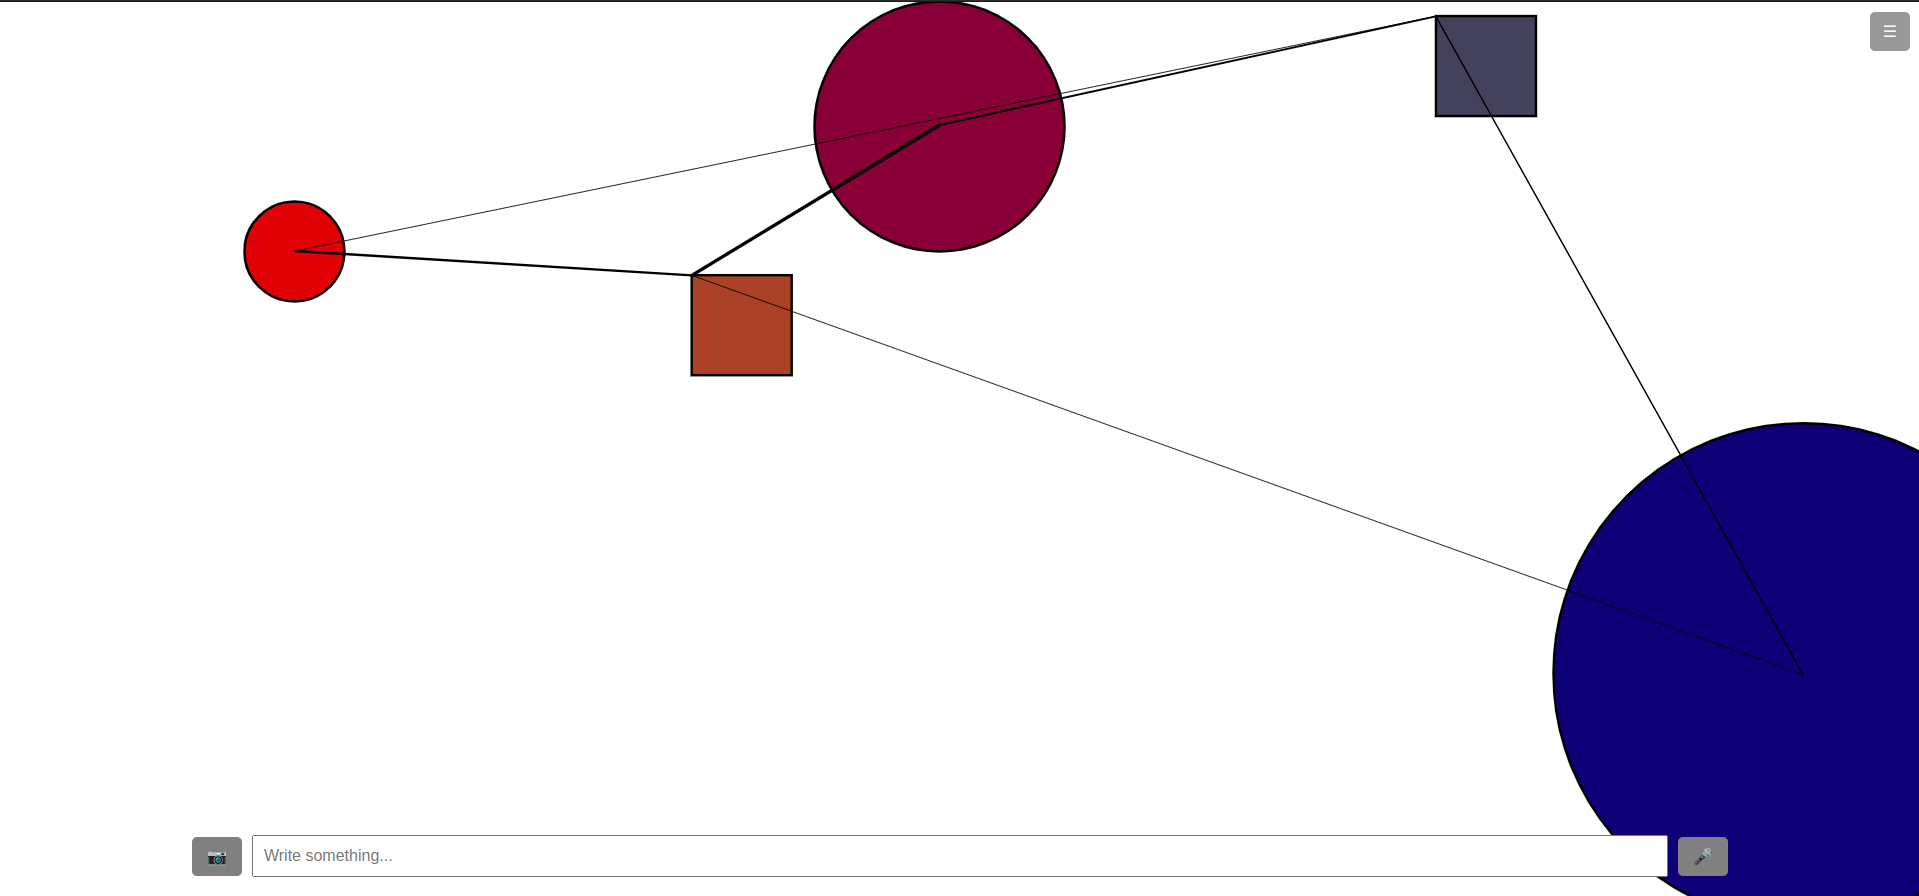
\includegraphics[width=\textwidth/3]{wbexp1.png}
    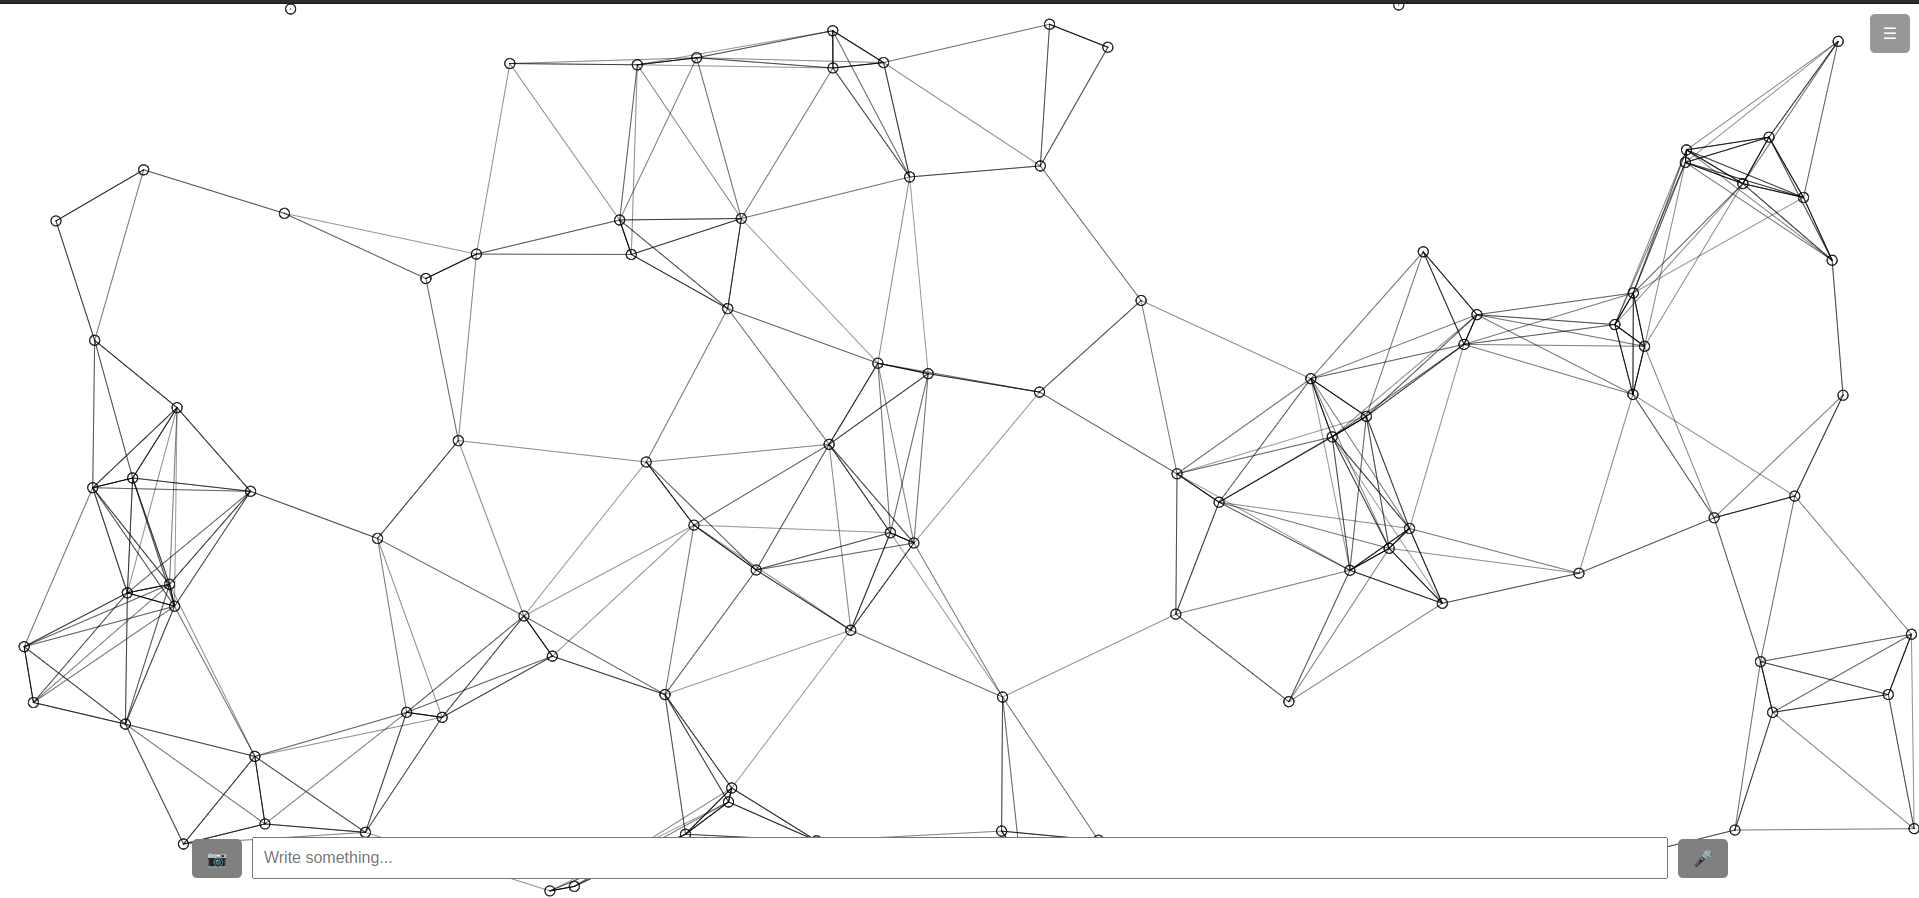
\includegraphics[width=\textwidth/3]{wbexp2.png}
    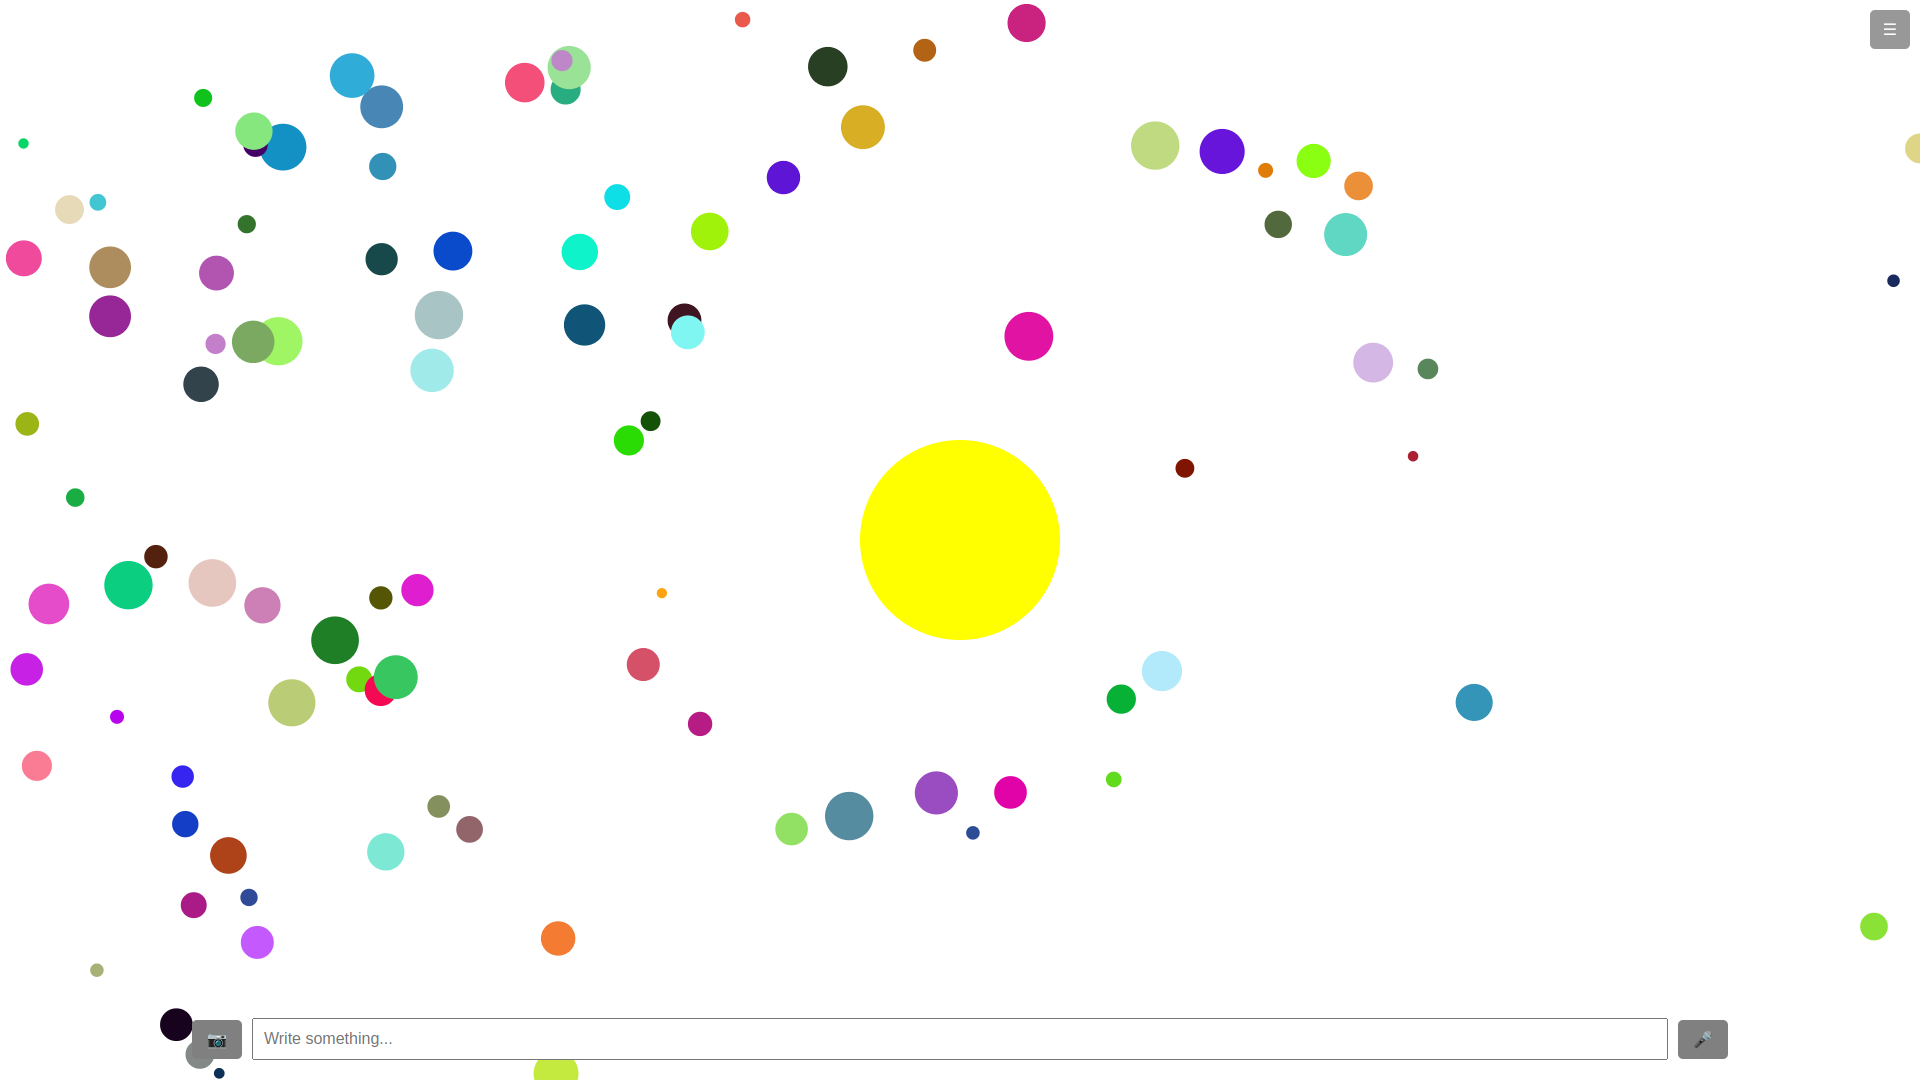
\includegraphics[width=\textwidth/3]{wbexp3.png}
    \caption{Demonstration of the LLM WhiteBoard in action.}
    \vspace{0.1cm}
    \label{fig:wbdemo1}
\end{figure}

\begin{figure}[h!]
    \centering
    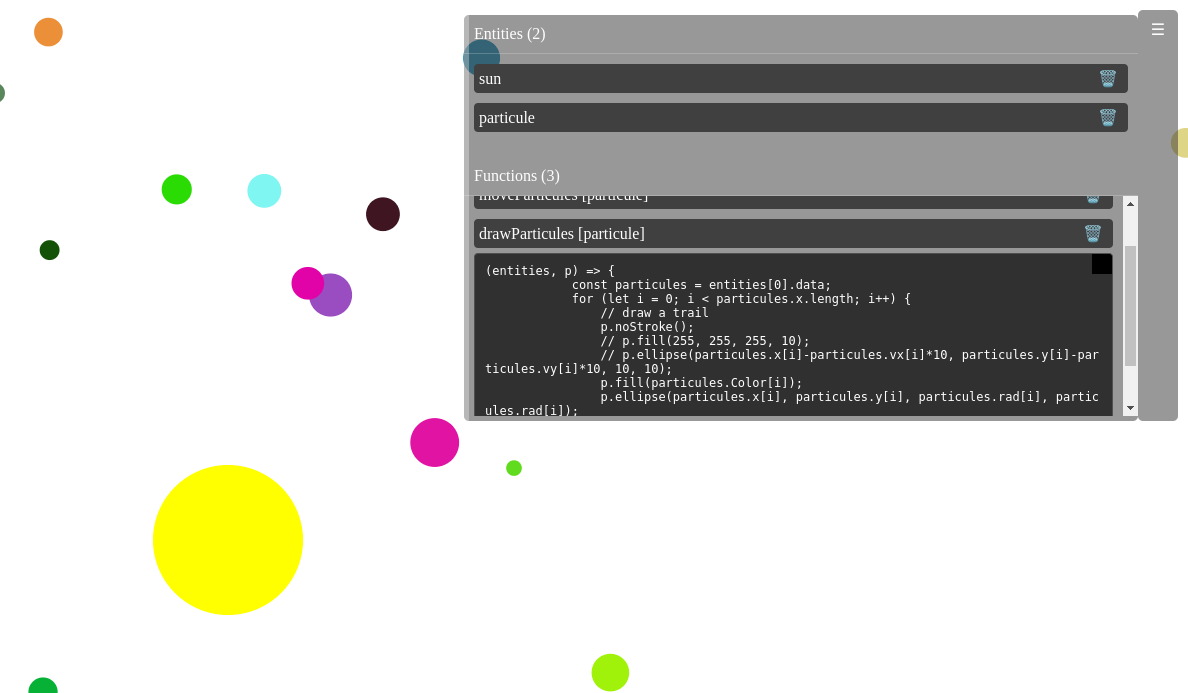
\includegraphics[width=\textwidth]{wbmenu.png}
    \caption{Menu allowing user to see the code generated by the LLM.}
    \vspace{0.1cm}
    \label{fig:wbmenu}
\end{figure}